\subsubsection{Kuratowskiho věta}
\label{sssec:kuratowskiho-veta}

Závěrem kapitoly o kreslení grafů a vlastně i závěrem celé části o teorii grafů
uvedeme zatím nejsilnější výsledek v celém textu, který dokonale charakterizuje
rovinné grafy. Jeho důkaz je těžký a dlouhý žádaje mnohých příprav.

V \hyperref[sssec:rovinne-grafy]{předchozí sekci} jsme tvrdili, že každý
nerovinný graf musí obsahovat $K_{3,3}$ nebo $K_5$. To není zcela korektní. Ve
skutečnosti musí obsahovat \emph{dělení} jednoho z těchto speciálních
nerovinných grafů jako podgraf. Ihned vysvětlíme,
co tento pojem znamená.

\begin{definition}[Dělení grafu]
 \label{def:deleni-grafu}
 Ať $G = (V,E)$ je graf. \emph{Dělením} grafu $G$ myslíme libovolný graf $H$,
 který vznikl z $G$ nějakým počtem opakování operace dělení hrany.
\end{definition}

Nyní můžeme vyslovit slavnou Kuratowskiho větu.

\begin{theorem}[Kuratowskiho]
 \label{thm:kuratowskiho}
 Graf $G$ je rovinný právě tehdy, když $G$ \textbf{neobsahuje} jako podgraf
 dělení $K_5$ ani dělení $K_{3,3}$.
\end{theorem}

\begin{figure}[h]
 \centering
 \begin{subfigure}[b]{.45\textwidth}
  \centering
  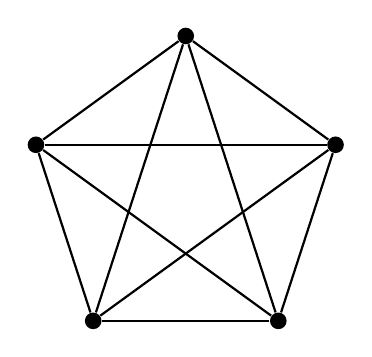
\begin{tikzpicture}[scale=2]
   \node[vertex] (a) at (18:1) {};
   \node[vertex] (b) at (90:1) {};
   \node[vertex] (c) at (162:1) {};
   \node[vertex] (d) at (234:1) {};
   \node[vertex] (e) at (306:1) {};

   \draw[thick] (a) -- (b);
   \draw[thick] (a) -- (c);
   \draw[thick] (a) -- (d);
   \draw[thick] (a) -- (e);
   \draw[thick] (b) -- (c);
   \draw[thick] (b) -- (d);
   \draw[thick] (b) -- (e);
   \draw[thick] (c) -- (d);
   \draw[thick] (c) -- (e);
   \draw[thick] (d) -- (e);
  \end{tikzpicture}
  \caption{Úplný graf $K_5$.}
  \label{subfig:k5}
 \end{subfigure}
 \begin{subfigure}[b]{.45\textwidth}
  \centering
   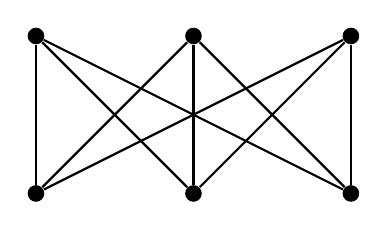
\begin{tikzpicture}[scale=2]
    \node[vertex] (a1) at (0,0) {};
    \node[vertex] (a2) at (1,0) {};
    \node[vertex] (a3) at (2,0) {};
    \node[vertex] (b1) at (0,-1) {};
    \node[vertex] (b2) at (1,-1) {};
    \node[vertex] (b3) at (2,-1) {};
    
    \draw[thick] (a1) -- (b1);
    \draw[thick] (a1) -- (b2);
    \draw[thick] (a1) -- (b3);
    \draw[thick] (a2) -- (b1);
    \draw[thick] (a2) -- (b2);
    \draw[thick] (a2) -- (b3);
    \draw[thick] (a3) -- (b1);
    \draw[thick] (a3) -- (b2);
    \draw[thick] (a3) -- (b3);
   \end{tikzpicture}
  \caption{Úplný bipartitní graf $K_{3,3}$.}
  \label{subfig:k33}
 \end{subfigure}
 \caption{Minimální nerovinné grafy.}
 \label{fig:minimalni-nerovinne-grafy}
\end{figure}

Je důležité podotknout, že \hyperref[thm:kuratowskiho]{Kuratowskiho věta} je
formulována jako \textbf{ekvivalence}. Tvrdí tudíž dvě věci:
\begin{itemize}
 \item Žádné dělení grafů $K_5$ a $K_{3,3}$ není rovinné.
 \item Každý nerovinný graf obsahuje jako podgraf aspoň jedno takové dělení.
\end{itemize}

Dokázat první bod není s přístupem k výsledkům
\hyperref[sssec:rovinne-grafy]{předchozí sekce} obtížné. Ukážeme nejprve, že
$K_{3,3}$ ani $K_5$ nejsou rovinné.

\begin{lemma}
 \label{lem:k33-k5-nerovinne}
 Grafy $K_5$ a $K_{3,3}$ nejsou rovinné.
\end{lemma}
\begin{proof}
 K důkazu obou tvrzení využijeme odhadu na počet hran rovinných grafů z
 \myref{lemmatu}{lem:hrany-rovinnych-grafu}.

 V případě $K_5$ stačí odhad $\# E \leq 3\# V - 6$. Totiž, $K_5$ má $5$ vrcholů
 a $\binom{5}{2} = 10$ hran. Ihned si všimneme, že $3 \cdot 5 - 6 = 9 < 10$, což
 znamená, že aspoň jeden pár hran se musí při nakreslení $K_5$ zkřížit, a tedy
 tento graf není rovinný.

 Graf $K_{3,3}$ má $3 + 3 = 6$ vrcholů a $3 \cdot 3 = 9$ hran. Tudíž splňuje
 slabší z odhadů v \myref{lemmatu}{lem:hrany-rovinnych-grafu}. Ovšem, všimněme
 si, že $K_{3,3}$ neobsahuje trojúhelníky. Vskutku, existence trojúhelníku
 $v_1v_2v_3v_1$ by znamenala existenci hrany $v_3v_1$ mezi dvěma vrcholy ze
 stejné části, což nelze. Můžeme tedy použít silnější odhad $\# E \leq 2\# V -
 4$, který již $K_{3,3}$ nesplňuje, poněvadž $2 \cdot 6 - 4 = 8 < 9$, tudíž je
 opět nutno při jeho kreslení zkřížit aspoň jeden pár hran.
\end{proof}

\hyperref[lem:k33-k5-nerovinne]{Předchozí lemma} doplníme o pár zřejmých
pozorování.

\begin{observation}
 Graf $G$ je rovinný právě tehdy, když každé jeho dělení je rovinné.
\end{observation}
\begin{proof}
 Zřejmý. Operace dělení hrany se v nakreslení grafu projeví náhradou křivky
 $\gamma$ křivkami $\gamma_1$ a $\gamma_2$, které lze vždy nakreslit tak, aby
 jejich spojením $\gamma_1\gamma_2$ byla původní křivka $\gamma$. Počet křížení
 hran při daném nakreslení tudíž zůstává nezměněn.
\end{proof}

\begin{observation}
 Každý podgraf $H$ rovinného grafu $G$ je rovinný.
\end{observation}
\begin{proof}
 Zřejmý. Vezměme libovolné rovinné nakreslení $G$ a vymažme všechny hrany a
 vrcholy, které nepatří do $H$. Získali jsme rovinné nakreslení $H$.
\end{proof}

Tato dvě pozorování společně s \myref{lemmatem}{lem:k33-k5-nerovinne} dávají
důkaz jedné implikace v \hyperref[thm:kuratowskiho]{Kuratowskiho větě}. Totiž,
ať $G$ je graf obsahující jako podgraf nějaké dělení $K_5$ nebo $K_{3,3}$. Podle
\myref{lemmatu}{lem:k33-k5-nerovinne} a prvního pozorování je toto dělení
nerovinný graf. Podle druhého pozorování $G$ rovněž není rovinný.

Jak pravichom, důkaz opačné implikace je výrazně obtížnější. Velmi hrubě řečeno
spočívá v nalezení maximálního cyklu v daném nerovinném grafu po odebrání jedné
křížící se hrany a v následné diskusi možných způsobů, jak zabránit tomu, aby
tato hrana mohla být dovnitř zvoleného cyklu (ne vně, neboť je maximální)
nakreslena bez křížení. Zjistíme, že vzniklé vzorce vrcholů a hran tvoříce tuto
zábranu již nutně definují graf, který je dělením $K_5$ nebo $K_{3,3}$.

Začneme pár dalšími definicemi.

\begin{definition}[Stupeň vrcholu]
 \label{def:stupen-vrcholu}
 Ať $G = (V,E)$ je graf. \emph{Stupeň vrcholu} $v \in V$ je počet hran, jímž
 náleží. Formálně,
 \[
  \deg_G v \coloneqq \# \{e \in E \mid v \in e\}.
 \]
\end{definition}

\begin{definition}[Řezný vrchol]
 \label{def:rezny-vrchol}
 Ať $G = (V,E)$ je graf. Vrchol $v \in V$ nazveme \emph{řezným}, pokud $G - v$
 má více komponent než $G$.
\end{definition}

Lidově řečeno, řezné vrcholy jsou takové vrcholy $G$, podle kterých jej můžeme
\uv{nařezat} na menší grafy.

\begin{definition}[Blok]
 \label{def:blok}
 Ať $G = (V,E)$ je graf. Podgraf $B$ grafu $G$ nazveme \emph{blokem}, pokud je
 to \textbf{maximální} podgraf $G$ bez řezných vrcholů. Slovo \uv{maximální} zde
 míní takový podgraf $B$, ke kterému když přidáme libovolný vrchol, který v něm
 neleží, bude už $B$ obsahovat řezný vrchol.
\end{definition}

\begin{definition}[2-souvislost]
 \label{def:2-souvislost}
 Graf $G = (V,E)$ nazveme \emph{2-souvislým}, pokud je souvislý a neobsahuje
 řezný vrchol. Tj. takový graf, který zůstane souvislým i po odebrání
 libovolného vrcholu.
\end{definition}

\begin{remark}
 Značení \uv{2-souvislý} může působit poněkud neintuitiv\-ně. Vlastně se jedná o
 speciální případ vlastnosti grafů zvané $k$-souvis\-lost. Ta se definuje tak,
 že graf je $k$-souvislý, kdykoli je souvislý a zůstane tak i po odebrání
 libovolných $k-1$ vrcholů.
\end{remark}

Dokážeme si dvě pomocná lemmata o $2$-souvislých grafech.

\begin{lemma}
 \label{lem:2-souvisly-cyklus}
 Ať $G = (V,E)$ je $2$-souvislý graf a $u,v \in V$. Pak v $G$ existuje cyklus
 obsahující $u$ i $v$.
\end{lemma}
\begin{proof}
 Budeme postupovat indukcí podle vzdálenosti mezi $u$ a $v$.

 Prvním indukčním krokem je případ $d_G(u,v) = 1$, tj. $uv \in E$. Uvažme graf
 $G - u$. Nejprve si všimněme, že $u$ musí mít aspoň dva sousedy, tj. stupeň
 aspoň 2. Kdyby tomu tak nebylo, byl by $v$ řezným vrcholem, neboť jeho vymazání
 by izolovalo vrchol $u$ od zbytku grafu. To by bylo ve sporu s předpokladem
 $2$-souvislosti $G$.

 Ať je tedy $w$ libovolný soused $u$ různý od $v$. Protože $G$ je $2$-souvislý,
 je $G - u$ souvislý. To znamená, že mezi $v$ a $w$ vede v $G - u$ cesta, která
 samozřejmě neobsahuje $u$, neboť jsme jej vyňali. Přidáním hrany $uv$ k~této
 cestě vznikne cyklus v $G$, který obsahuje $u$ i $v$.

 Nyní předpokládejme, že $d_G(u,v) = d$ a tvrzení platí pro všechny dvojice
 vrcholů se vzdáleností ostře menší než $d$. Ať $P$ je cesta délky $d$ mezi $u$
 a $v$ a $w$ je předposlední vrchol na této cestě (tedy soused $v$, který leží
 na $P$). Jelikož $d_G(u,w) = d - 1$, existuje z indukčního předpokladu cyklus
 $C$ obsahující $u$ i $w$. Dále, $G - w$ je souvislý, a tedy v~něm existuje
 cesta $Q$ mezi $u$ a $v$, která samozřejmě neprochází vrcholem $w$. Střídavým
 sledováním vrcholů cyklu $C$ a cesty $Q$ tak, aby se žádné neopakovaly,
 dostaneme cyklus obsahující $u$ a $v$.

 Formální zápis poslední věty je extrémně zdlouhavý a nepřináší užitečné ideje.
 Pro lepší představu vizte \myref{obrázek}{fig:2-souvisly-cyklus}.
\end{proof}

\begin{figure}[h]
 \centering
 \begin{tikzpicture}[scale=2]
  \pgfdeclarelayer{background}
  \pgfsetlayers{background,main}

  \draw[thick,myred] (0,0) ellipse (2 and 1);
  \node[vertex,myblue] (u) at (-2,0) {};
  \node[vertex,mypurple] (v) at (2,0) {};
  \node[vertex,below right=0.5 and 1 of v,myblue] (w) {};
  \node[vertex] (r1) at (-1.37,0.73) {};
  \node[vertex] (r2) at (-0.4,-0.98) {};
  \node[vertex] (r3) at (0.97,-0.88) {};
  \node[vertex] (r4) at (1.54,-0.64) {};

  \node[below left=-1mm and -1mm of u,myblue] {\large $u$};
  \node[above right=-1mm and -1mm of v,mypurple] {\large $w$};
  \node[right=0mm of w,myblue] {\large $v$};

  \node at (-2,0.95) {$Q$};
  \node[myred] at (1.6,0.8) {$C$};
  \begin{pgfonlayer}{background}
   \draw[thick] (u) .. controls (-2.5,0.5) and (-2,1) .. (r1);
   \draw[thick] (r1) .. controls (-0.2,0) and (-1,0) .. (r2);
   \draw[thick] (r2) .. controls (0.1,-1.7) and (0.77,-1.6) .. (r3);
   \draw[thick] (r3) .. controls (1,-0.58) and (1.24,-0.44) .. (r4);
   \draw[thick] (r4) .. controls (1.64,-0.74) and (2,-1) .. (w);
   \draw[thick] (w) -- (v);
  \end{pgfonlayer}
 \end{tikzpicture}

 \caption{Konec důkazu \myref{lemmatu}{lem:2-souvisly-cyklus}. Sledováním
  obrázku po obvodu dostaneme cyklus obsahující $\clb{u}$ a $\clb{v}$ složený z
  vrcholů cyklu $\clr{C}$ a cesty $Q$.}
 \label{fig:2-souvisly-cyklus}
\end{figure}

\begin{definition}[Ucho]
 \label{def:ucho}
 Ať $G = (V,E)$ je graf a $H = (V',E')$ jeho podgraf. \emph{Uchem} v grafu $G$
 ke grafu $H$ myslíme cestu $e_1e_2\cdots e_n$, kde $e_i \in E$, takovou, že
 $s(e_1), t(e_n) \in V'$, ale $e_i \notin E'$ pro každé $i \leq n$. Je to tedy
 vlastně cesta, která začíná a končí v $H$, ale jinak jím neprochází.
\end{definition}

\begin{lemma}
 \label{lem:konstrukce-pres-ucha}
 Každý $2$-souvislý graf lze zkonstruovat z cyklu přidáváním uch.
\end{lemma}
\begin{proof}
 Ať $G = (V,E)$ je graf vzniklý touto konstrukcí. Dokážeme, že $G$ je
 $2$-souvislý. Budeme postupovat indukcí podle počtu přidaných uch. Nepřidali-li
 jsme ani jedno ucho, pak je $G$ cyklus, který je jistě $2$-souvislý. Nyní ať
 $U$ je nově přidané ucho ke $G$ a $u_1,u_2 \in V$ jsou vrcholy, kterými je $U$
 ke $G$ připojeno. Protože $G$ byl z indukčního předpokladu $2$-souvislý, musí
 případný řezný vrchol ležet na $U$. Předpokládejme pro spor tedy, že takový
 existuje, a označme ho $v \in U$. Rozlišíme dva případy:
 \begin{enumerate}
  \item $v \notin V$; v takovém případě byl $v$ součástí cyklu, který získáme
   tak, že spojíme cestu mezi $u_1$ a $u_2$ v $G$ s nově přidaných uchem $U$.
   Protože má navíc $v$ jen dva sousedy, nemůže jeho odebrání graf rozpojit.
  \item $v \in \{u_1,u_2\}$; v tomto případě není $v$ řezným v $U$ (protože je
   na jeho konci) a není z předpokladu $2$-souvislosti řezný ani v $G$. Tudíž
   není řezný ani v grafu $G$ sloučeném s uchem $U$.
 \end{enumerate}

 Pokračujeme důkazem, že \textbf{každý} $2$-souvislý graf $G = (V,E)$ lze takto
 postavit. Podle \myref{lemmatu}{lem:2-souvisly-cyklus} $G$ obsahuje cyklus.
 Vezměme maximální podgraf $H = (V',E')$ grafu $G$, který lze přidáváním uch
 zkonstruovat. K důkazu stačí ověřit, že $H$ už je celý graf $G$. Platí, že
 \begin{itemize}
  \item $H$ je indukovaný podgraf. Vskutku, pokud $H$ indukovaný není, pak
   existuje hrana $e \in E$, která spojuje dva vrcholy z $H$, ale sama v $H$
   neleží. Z \hyperref[def:ucho]{definice} je taková hrana ucho k $H$, což je
   spor s~maximalitou $H$.
  \item $H = G$. Pro spor ať toto neplatí. Uvažme hranu $uv \in E$ takovou, že
   $u \in V'$ a $v \in V \setminus V'$, tedy takovou, že její začátek leží v $H$
   a konec mimo $H$. Taková hrana určitě existuje, neboť $G$ je souvislý, a
   tudíž $H$ nemůže být komponenta $G$. Navíc, $G$ je též $2$-souvislý, pročež
   existuje cyklus (opět z \myref{lemmatu}{lem:2-souvisly-cyklus}) obsahující
   $u$ a $v$. Odebereme-li z tohoto cyklu všechny hrany, které neleží v $E'$,
   dostaneme ucho k grafu $H$ a tím opět spor s maximalitou tohoto podgrafu.
 \end{itemize}
 Jelikož $H$ vznikl z předpokladu přidáváním uch k cyklu a platí $H = G$, důkaz
 je hotov.
\end{proof}

\begin{figure}[h]
 \centering
 \begin{tikzpicture}
  \pgfdeclarelayer{background}
  \pgfsetlayers{background,main}
  \node[vertex] (c1) at (30:1.512) {};
  \node[vertex] (c2) at (90:1) {};
  \node[vertex] (c3) at (144:1.401) {};
  \node[vertex] (c4) at (180:2) {};
  \node[vertex] (c5) at (292.5:1.06) {};
  \node[vertex] (c6) at (-18:1.763) {};

  \node[vertex,myred] (a1) at (52:3) {};
  \node[vertex,myred] (a2) at (15:4) {};
  \node[vertex,myred] (a3) at (-10:3.5) {};

  \node[vertex,myblue] (b1) at (75:4) {};
  \node[vertex,myblue] (b2) at (110:4) {};
  \node[vertex,myblue] (b3) at (150:3) {};
  \begin{pgfonlayer}{background}
   \draw[thick] (0,0) ellipse (2 and 1);
   \draw[thick,myred] plot [smooth] coordinates {(c2) (a1) (a2) (a3) (c6)};
   \draw[thick,myblue] plot [smooth] coordinates {(a1) (b1) (b2) (b3) (c4)};
  \end{pgfonlayer}
 \end{tikzpicture}

 \caption{Konstrukce z \myref{lemmatu}{lem:konstrukce-pres-ucha}.}
 \label{fig:konstrukce-pres-ucha}
\end{figure}

Konečně jsme splnili veškerou přípravu nutnou k důkazu Kuratowskiho věty. Těžkou
implikaci dokážeme sporem. Budeme předpokládat, že existuje nerovinný graf $G =
(V,E)$, který \textbf{neobsahuje} dělení $K_5$ ani $K_{3,3}$. Navíc, ze všech
takových grafů si vezmeme ten minimální co do počtu vrcholů a hran. Tím myslíme,
že pro každý $v \in V$ a pro každou $e \in E$ jsou již grafy $G - v$ a $G - e$
rovinné. Ukážeme, že takový minimální graf $G$ musí splňovat jisté striktní
podmínky, které nakonec povedou k závěru, že ve skutečnosti obsahuje dělení
$K_5$ nebo $K_{3,3}$, což bude přímý spor s předpokladem.

Následující důkaz v průběhu doplníme pomocnými lemmaty a tvrzeními, neboť psát
ho celý bez přerušení by bylo velmi nepřehledné a vyčerpávající.

\begin{enhproof}[{\hyperref[thm:kuratowskiho]{Kuratowskiho věty}}]
 Implikaci zleva doprava jsme již diskutovali výše. Obsahuje-li graf $G$ dělení
 $K_5$ nebo $K_{3,3}$ jako podgraf, pak není rovinný.

 Dokazujme tedy, že každý nerovinný graf musí obsahovat dělení $K_5$ nebo
 $K_{3,3}$. Mějme zvolený minimální nerovinný graf $G = (V,E)$, který neobsahuje
 dělení $K_5$ ani $K_{3,3}$ z úvahy nad důkazem.\\

 \hrule

 \begin{auxilprop}
  \label{auxilprop:graf-rovinny-iff-bloky-rovinne}
  Graf $H$ je rovinný právě tehdy, když každý jeho blok je rovinný.
 \end{auxilprop}
 \textbf{\sffamily Důkaz.} Je-li $H$ rovinný, pak je každý jeho podgraf
 rovinný, tedy speciálně i každý jeho blok je rovinný.

 Nechť naopak je každý blok $H$ rovinný. Nejprve si uvědomíme, že dva různé
 bloky se pronikají v maximálně jednom vrcholu (který je tím pádem řezný v
 grafu $H$). Kdyby totiž v jejich průniku byly dva nebo více, pak bychom mohli
 jeden z nich odebrat a bloky bychom tím neoddělili; to by znamenalo, že jejich
 sloučení byl $2$-souvislý graf, což je spor s definicí bloku jako maximálního
 $2$-souvislého podgrafu.

 Dále postupujme indukcí podle počtu bloků grafu $H$. Když má $H$ jeden blok,
 tak tvrzení zřejmě platí.

 V druhém indukčním kroku uvažujme, že $H$ má $n \in \N$ různých bloků. Mezi
 nimi musí existovat aspoň jeden blok $B$, který sousedí pouze s~jedním dalším
 (tedy s ním sdílí vrchol nebo je s ním spojen cestou). Kdyby tomu taky nebylo,
 tak by každý blok byl součástí cyklu bloků (neboť by každý blok měl aspoň dva
 sousedy). Je snadné nahlédnout, že cyklus bloků je $2$-souvislý graf a
 dostáváme opět spor s maximalitou bloků.

 Uvažme graf $H'$ vzniklý z $H$ odebráním všech vrcholů z $B$ kromě případného
 vrcholu v průniku $B$ s jeho sousedem. Graf $H'$ má o jeden blok méně než $H$,
 čili je z indukčního předpokladu rovinný. Nyní nakreslíme $H'$ tak, aby onen
 vrchol spojující $H'$ a $B$ byl součástí vnější stěny (to zřejmě vždy lze).
 Blok $B$ dokreslíme rovněž na vnější stěně, čímž získáme rovinné nakreslení
 $H$.\hfill\qed\\

 \hrule

 \begin{figure}[H]
  \centering
  \begin{tikzpicture}
   \draw[thick] (0,0) ellipse (2 and 1);
   \draw[thick] (-2,2.5) circle (0.8);
   \node at (0,0) {\large $H'$};
   \node at (-2,2.5) {\large $B$};

   \node[vertex] (a) at (-1.08, 0.84) {};
   \node[vertex] (b) at (-1.6,1.81) {};

   \draw[thick,snake it] (a) -- (b);
   
  \end{tikzpicture}

  \caption{Indukční krok v důkazu \myref{pomocného
   tvrzení}{auxilprop:graf-rovinny-iff-bloky-rovinne}.}
  \label{fig:graf-rovinny-iff-bloky-rovinne}
 \end{figure}

 Připomeňme, že stále pracujeme s fixním minimální nerovinným grafem $G$
 neobsahujícím dělení ani $K_5$ ani $K_{3,3}$.\\

 \hrule

 \begin{auxilprop}
  \label{auxilprop:G-2-souvisly}
  $G$ je nutně $2$-souvislý.
 \end{auxilprop}
 \textbf{\sffamily Důkaz.} Předpokládejme, že $G$ $2$-souvislý není. Pak podle
 \myref{pomocného tvrzení}{auxilprop:graf-rovinny-iff-bloky-rovinne} obsahuje
 nějaký nerovinný blok. Pokud by tento blok nebyl celý graf $G$, pak bychom
 našli menší nerovinný graf neobsahující dělení $K_5$ ani $K_{3,3}$, což by byl
 spor s minimalitou $G$. Tedy, $G$ sám je blok, a tudíž je $2$-souvislý z
 definice.\hfill\qed\\

 \hrule

 \begin{auxilprop}
  \label{auxilprop:G-nema-stupen-2}
  $G$ neobsahuje vrchol stupně menšího než $3$.
 \end{auxilprop}
 \textbf{\sffamily Důkaz.} $G$ neobsahuje vrchol stupně $0$, neboť je souvislý.
 Podobně, $G$ neobsahuje ani žádný vrchol stupně $1$, protože libovolný soused
 takového vrcholu by byl řezný, a tudíž by $G$ nebyl $2$-souvislý, což by
 znamenalo spor s \myref{pomocným tvrzením}{auxilprop:G-2-souvisly}.

 Zbývá ukázat, že $G$ neobsahuje ani vrchol stupně $2$. Uvažme tudíž pro spor
 nějaký vrchol $u$ stupně $2$ a označme $v,w$ jeho dva sousedy. Rozlišíme dva
 případy.
 \begin{enumerate}
  \item Existuje hrana $vw \in E$, tj. $v$ a $w$ jsou sousedi. Z předpokladu
   minimality $G$ je graf $G - u$ rovinný. Zvolme tedy nějaké jeho rovinné
   nakreslení. K tomuto nakreslení lze přikreslit cestu $vuw$ libovolně blízko
   hraně $vw$ aniž dojde ke křížení. To ale znamená, že $G$ má rovinné
   nakreslení, což je spor.
  \item Hrana $vw$ neexistuje. Smažme vrchol $u$ a přidejme hranu $vw$. Vzniklý
   graf má o jednu hranu a jeden vrchol méně než $G$, a tedy je z předpokladu
   rovinný. Ovšem, v libovolném rovinném nakreslení tohoto grafu, můžeme
   rozdělit hranu $vw$ a tím získat zpět smazaný vrchol $u$. Již jsme
   zpozorovali, že dělení rovinného grafu je rovinné, tudíž získáváme opět spor
   s tím, že $G$ není rovinný.
 \end{enumerate}
 V obou případech jsme došli ke sporu, pročež každý vrchol $G$ má stupeň alespoň
 $3$.\hfill\qed\\

 \hrule

 \begin{figure}[H]
  \centering
  \begin{subfigure}{.45\textwidth}
   \centering
   \begin{tikzpicture}[scale=1.5]
    \node[vertex] (v) at (0,0) {};
    \node[vertex,myred] (u) at (0.8,0.5) {};
    \node[vertex] (w) at (1,1) {};
    \node[vertex] (r1) at (2,2) {};
    \node[vertex] (r2) at (0,2) {};
    
    \node[left=0mm of v] {$v$};
    \node[below right=-1mm and -1mm of u,myred] {$u$};
    \node[right=0mm of w] {$w$};

    \draw[thick] (v) -- (w);
    \draw[thick] (w) -- (r1);
    \draw[thick] (w) -- (r2);
    \draw[thick] (r1) -- (r2);
    \draw[thick] (v) -- (r2);
    \draw[thick,myred] (v) -- (u);
    \draw[thick,myred] (u) -- (w);
   \end{tikzpicture}
   \caption{Případ (1).}
   \label{subfig:G-nema-stupen-2-pripad-1}
  \end{subfigure}
  \begin{subfigure}{.45\textwidth}
   \centering
    \begin{tikzpicture}[scale=1.5]
     \node[vertex] (v) at (0,0) {};
     \node[vertex,myred] (u) at (0.5,0.5) {};
     \node[vertex] (w) at (1,1) {};
     \node[vertex] (r1) at (1,2) {};
     \node[vertex] (r2) at (-0.5,1) {};
     \node[vertex] (r3) at (-0.7,1.5) {};

     \node[left=0mm of v] {$v$};
     \node[below right=-1mm and -1mm of u,myred] {$u$};
     \node[right=0mm of w] {$w$};

     \draw[thick] (w) -- (r1);
     \draw[thick] (r1) -- (r3);
     \draw[thick] (r3) -- (r2);
     \draw[thick] (r2) -- (r1);
     \draw[thick] (v) -- (r2);
     \draw[thick,myred] (v) -- (u);
     \draw[thick,myred] (u) -- (w);
    \end{tikzpicture}
   \caption{Případ (2).}
   \label{subfig:G-nema-stupen-2-pripad-2}
  \end{subfigure}
  \caption{Důkaz \myref{pomocného tvrzení}{auxilprop:G-nema-stupen-2}.}
  \label{fig:G-nema-stupen-2}
 \end{figure}

 \begin{auxilprop}
  \label{auxilprop:G-bez-uv-2-souvisly}
  $G$ má hranu $e \in E$ takovou, že $G - e$ je stále $2$-souvislý.
 \end{auxilprop}
 \textbf{\sffamily Důkaz.} Podle \myref{lemmatu}{lem:konstrukce-pres-ucha}
 vznikl $G$ opakovaným přidáváním uch k cyklu. Ať $U$ značí poslední přidané
 ucho. Má-li $U$ délku aspoň dva, pak v něm existuje vrchol stupně $2$, což je
 spor s \myref{pomocným tvrzením}{auxilprop:G-nema-stupen-2}. Odtud plyne, že
 $U$ musí být pouze jediná hrana $e \in E$. Pak je $G - e$ zřejmě stále
 $2$-souvislý (neboť též vznikl přidáváním uch k~cyklu).\hfill\qed\\

 \hrule

 Pomalu ale jistě se blížíme ke konci důkazu. Ať $H \coloneqq G - uv$, kde $uv
 \in E$ je hrana $G$ taková, že $G - uv$ je stále $2$-souvislý (jejíž existence
 je zaručena \myref{pomocným tvrzením}{auxilprop:G-bez-uv-2-souvisly}). Protože
 $G$ byl minimální nerovinný, je $H$ z předpokladu rovinný graf. Dále, $H$ je
 $2$-souvislý, a tudíž v něm, podle \myref{lemmatu}{lem:2-souvisly-cyklus},
 existuje aspoň jeden cyklus obsahující $u$ i $v$.

 Nyní volme takové rovinné nakreslení $D$ grafu $H$, že obsahuje cyklus $C$
 splňující:
 \begin{itemize}
  \item $C$ obsahuje $u$ i $v$.
  \item Počet stěn uvnitř $C$ je maximální přes všechna možná rovinná
   nakreslení.
  \item Je-li $C'$ jiný cyklus obsahující $u$ i $v$, pak počet stěn uvnitř $C'$
   v~libovolném nakreslení $H$ je menší nebo roven počtu stěn v $C$.
 \end{itemize}

 Shrňme v lidském jazyce, co poslední dva body říkají. Volíme cyklus $C$ a
 nakreslení $D$ takové, že počet stěn uvnitř $C$ je maximální přes
 \textbf{všechny} cykly obsahující $u$ a $v$, přes \textbf{všechna} možná
 rovinná nakreslení $H$. Ještě jinak řečeno, kdykoli nakreslíme $H$ jakýmkoli
 rovinným způsobem a zvolíme v něm jakýkoli cyklus obsahující $u$ a $v$, tak
 tento cyklus bude mít uvnitř nejvíce tolik stěn jako $C$ při nakreslení $D$.

 Označme
 \[
  C = (u = v_0)v_1v_2 \cdots (v_k = v)v_{k+1}\cdots v_lv_0.
 \]
 Jistě platí $k \geq 2$, neboť hranu $uv$ jsme odebrali. Pozorujeme, že
 \begin{itemize}
  \item neexistuje žádná cesta spojující dva vrcholy z $\{v_0,\ldots,v_k\}$,
   která leží vně $C$;
  \item neexistuje žádná cesta spojující dva vrcholy z
   $\{v_k,v_{k+1},\ldots,v_l,v_0\}$, která leží vně $C$.
 \end{itemize}
 Vskutku, uvažme, že by existovala cesta $P$ spojující dva vrcholy $v_i,v_j$
 třeba z první množiny, která by ležela vně $C$. Pak by přeci cyklus
 \[
  v_0v_1\cdots v_iPv_jv_{j+1}\cdots v_lv_0
 \] 
 obsahoval $u$ i $v$ a uvnitř aspoň o jednu stěnu víc než $C$ (vizte
 \myref{obrázek}{fig:cesta-mezi-vi-a-vj}). Tím bychom dostali spor s maximalitou
 $C$.

 \begin{figure}[H]
  \centering
  \begin{tikzpicture}
   \pgfdeclarelayer{background}
   \pgfsetlayers{background,main}
   \node[vertex,myred] (vj) at (30:1.512) {};
   \node[vertex] (c2) at (90:1) {};
   \node[vertex,myred] (vi) at (144:1.401) {};
   \node[vertex] (u) at (180:2) {};
   \node[vertex] (c5) at (292.5:1.06) {};
   \node[vertex] (c6) at (-18:1.763) {};
   \node[vertex] (v) at (0:2) {};

   \node[left=0 of u] {$u = v_0$};
   \node[right=0 of v] {$v_k = v$};
   \node[above left=-1mm and -1mm of vi,myred] {$v_i$};
   \node[above right=-2mm and -1mm of vj,myred] {$v_j$};

   \node (r) at (85:2) {};
   \node[above=-1mm of r,myblue] {$P$};
   
   \begin{pgfonlayer}{background}
    \draw[thick] (0,0) ellipse (2 and 1);
    \draw[thick,myblue] plot [smooth,tension=2] coordinates {(vi) (r) (vj)};
   \end{pgfonlayer}
  \end{tikzpicture}

  \caption{Cesta $\clb{P}$ spojující vrcholy $\clr{v_i}$ a $\clr{v_j}$.}
  \label{fig:cesta-mezi-vi-a-vj}
 \end{figure}

 Z předpokladu minimality $G$ nelze přikreslit hranu $uv$ ke zvolenému
 nakreslení $H$ bez křížení. To ovšem znamená, že musí existovat cesta, která,
 spojujíc dva vrcholy cyklu $C$, ležíc mimo něj a \uv{obklopujíc} buď vrchol $u$
 nebo vrchol $v$, brání tomuto přikreslení.

 Konkrétně, musí existovat cesta $Q$ spojující vrchol z $\{v_1,\ldots,v_{k-1}\}$
 s vrcholem z $\{v_{k+1},\ldots,v_l\}$ nakreslená vně cyklu $C$ jako na
 \myref{obrázku}{fig:cesta-vne-cyklu}.

 \begin{figure}[H]
  \centering
  \begin{tikzpicture}
   \pgfdeclarelayer{background}
   \pgfsetlayers{background,main}
   \node[vertex] (vj) at (30:1.512) {};
   \node[vertex] (c2) at (90:1) {};
   \node[vertex] (vi) at (144:1.401) {};
   \node[vertex] (u) at (180:2) {};
   \node[vertex] (c5) at (292.5:1.06) {};
   \node[vertex] (c6) at (-18:1.763) {};
   \node[vertex] (v) at (0:2) {};
   \node[above left=-1mm and -1mm of c2] {$v_2$};
   \node[below left=-1mm and -1mm of c5] {$v_l$};

   \node[left=0 of u] {$u = v_0$};
   \node[right=0 of v] {$v_k = v$};

   \node (r1) at (60:3) {};
   \node (r2) at (0:4) {};
   \node (r3) at (-50:3) {};
   \node[right=0mm of r2,myblue] {$Q$};

   \begin{pgfonlayer}{background}
    \draw[thick] (0,0) ellipse (2 and 1);
    \draw[thick,myblue] plot [smooth,tension=1] coordinates {(c2) (r1) (r2) (r3)
     (c5)};
   \end{pgfonlayer}
  \end{tikzpicture}

  \caption{Cesta $\clb{Q}$ bránící přikreslení hrany $uv$.}
  \label{fig:cesta-vne-cyklu}
 \end{figure}

 Dále, tato cesta $Q$ nemůže být nakreslena bez křížení uvnitř cyklu $C$, jinak
 by existovalo nakreslení $H$, kam by bylo lze hranu $uv$ přikreslit vně $C$ a
 získat tak rovinné nakreslení $G$. To ovšem znamená, že navíc musí existovat
 nějaká struktura uvnitř cyklu $C$, která brání nakreslení cesty $Q$. Taková
 struktura musí v zásadě neumožnit průchod od vrcholu $u$ do vrcholu $v$
 vnitřkem cyklu $C$.

 Není obtížné si rozmyslet (\textbf{zkuste si to!}), že ona struktura nabývá
 nutně jedné ze čtyř podob na \myref{obrázku}{fig:struktury-uvnitr-C}.

 \begin{figure}[H]
  \tikzset{
    vertex/.style = {shape=circle,fill,text=white,minimum size=6pt,inner
    sep=1pt}
  }
  \centering
  \begin{subfigure}[b]{.49\textwidth}
   \centering
   \begin{tikzpicture}[scale=0.65]
    \pgfdeclarelayer{background}
    \pgfsetlayers{background,main}
    \node[vertex] (vj) at (30:1.512) {};
    \node[vertex] (c2) at (90:1) {};
    \node[vertex] (vi) at (144:1.401) {};
    \node[vertex] (u) at (180:2) {};
    \node[vertex] (c5) at (292.5:1.06) {};
    \node[vertex] (c6) at (-18:1.763) {};
    \node[vertex] (v) at (0:2) {};
    \node[above left=-1mm and -1mm of c2] {\small $v_2$};
    \node[below left=-1mm and -1mm of c5] {\small $v_l$};

    \node[left=0 of u] {\small $u = v_0$};
    \node[right=0 of v] {\small $v_k = v$};

    \node (r1) at (60:3.5) {};
    \node (r2) at (0:4.5) {};
    \node (r3) at (-50:3) {};
    \node[right=2mm of r1,myblue] {\small $Q$};

    \begin{pgfonlayer}{background}
     \draw[thick] (0,0) ellipse (2 and 1);
     \draw[thick,myblue] plot [smooth,tension=1] coordinates {(c2) (r1) (r2) (r3)
      (c5)};
     \draw[thick,snake it] (vi) -- (c6);
    \end{pgfonlayer}
   \end{tikzpicture}
   \caption{Případ 1.}
   \label{subfig:struktury-uvnitr-C-1}
  \end{subfigure}
  \hfill
  \begin{subfigure}[b]{.49\textwidth}
   \centering
   \begin{tikzpicture}[scale=0.65]
    \pgfdeclarelayer{background}
    \pgfsetlayers{background,main}
    \node[vertex] (vj) at (30:1.512) {};
    \node[vertex] (c2) at (90:1) {};
    \node[vertex] (vi) at (144:1.401) {};
    \node[vertex] (u) at (180:2) {};
    \node[vertex] (c5) at (292.5:1.06) {};
    \node[vertex] (c6) at (-18:1.763) {};
    \node[vertex] (v) at (0:2) {};
    \node[above left=-1mm and -1mm of c2] {\small $v_2$};
    \node[below left=-1mm and -1mm of c5] {\small $v_l$};

    \node[left=0 of u] {\small $u = v_0$};
    \node[right=0 of v] {\small $v_k = v$};

    \node (r1) at (60:3.5) {};
    \node (r2) at (0:4.5) {};
    \node (r3) at (-50:3) {};
    \node[right=2mm of r1,myblue] {\small $Q$};

    \node[vertex] (c) at (0,0) {};    

    \begin{pgfonlayer}{background}
     \draw[thick] (0,0) ellipse (2 and 1);
     \draw[thick,myblue] plot [smooth,tension=1] coordinates {(c2) (r1) (r2) (r3)
      (c5)};
     \draw[thick,snake it] (u) -- (c);
     \draw[thick,snake it] (c) -- (vj);
     \draw[thick, snake it] (c) -- (c6);
    \end{pgfonlayer}
   \end{tikzpicture}
   \caption{Případ 2.}
   \label{subfig:struktury-uvnitr-C-2}
  \end{subfigure}
  \begin{subfigure}[b]{.49\textwidth}
   \centering
   \begin{tikzpicture}[scale=0.65]
    \pgfdeclarelayer{background}
    \pgfsetlayers{background,main}
    \node[vertex] (vj) at (30:1.512) {};
    \node[vertex] (c2) at (90:1) {};
    \node[vertex] (vi) at (144:1.401) {};
    \node[vertex] (u) at (180:2) {};
    \node[vertex] (c5) at (292.5:1.06) {};
    \node[vertex] (c6) at (-18:1.763) {};
    \node[vertex] (v) at (0:2) {};
    \node[above left=-1mm and -1mm of c2] {\small $v_2$};
    \node[below left=-1mm and -1mm of c5] {\small $v_l$};

    \node[left=0 of u] {\small $u = v_0$};
    \node[right=0 of v] {\small $v_k = v$};

    \node (r1) at (60:3.5) {};
    \node (r2) at (0:4.5) {};
    \node (r3) at (-50:3) {};
    \node[right=2mm of r1,myblue] {\small $Q$};

    \node[vertex] (d1) at (-1,0) {};    
    \node[vertex] (d2) at (1,0) {};    

    \begin{pgfonlayer}{background}
     \draw[thick] (0,0) ellipse (2 and 1);
     \draw[thick,myblue] plot [smooth,tension=1] coordinates {(c2) (r1) (r2) (r3)
      (c5)};
     \draw[thick,snake it] (u) -- (d1);
     \draw[thick,snake it] (d1) -- (c5);
     \draw[thick,snake it] (d1) -- (d2);
     \draw[thick,snake it] (d2) -- (c2);
     \draw[thick, snake it] (d2) -- (v);
    \end{pgfonlayer}
   \end{tikzpicture}
   \caption{Případ 3.}
   \label{subfig:struktury-uvnitr-C-3}
  \end{subfigure}
  \begin{subfigure}[b]{.49\textwidth}
   \centering
   \begin{tikzpicture}[scale=0.65]
    \pgfdeclarelayer{background}
    \pgfsetlayers{background,main}
    \node[vertex] (vj) at (30:1.512) {};
    \node[vertex] (c2) at (90:1) {};
    \node[vertex] (vi) at (144:1.401) {};
    \node[vertex] (u) at (180:2) {};
    \node[vertex] (c5) at (292.5:1.06) {};
    \node[vertex] (c6) at (-18:1.763) {};
    \node[vertex] (v) at (0:2) {};
    \node[above left=-1mm and -1mm of c2] {\small $v_2$};
    \node[below left=-1mm and -1mm of c5] {\small $v_l$};

    \node[left=0 of u] {\small $u = v_0$};
    \node[right=0 of v] {\small $v_k = v$};

    \node (r1) at (60:3.5) {};
    \node (r2) at (0:4.5) {};
    \node (r3) at (-50:3) {};
    \node[right=2mm of r1,myblue] {\small $Q$};

    \node[vertex] (c) at (0,0) {};    

    \begin{pgfonlayer}{background}
     \draw[thick] (0,0) ellipse (2 and 1);
     \draw[thick,myblue] plot [smooth,tension=1] coordinates {(c2) (r1) (r2) (r3)
      (c5)};
     \draw[thick,snake it] (u) -- (c);
     \draw[thick,snake it] (c) -- (c2);
     \draw[thick,snake it] (c) -- (c5);
     \draw[thick,snake it] (c) -- (v);
    \end{pgfonlayer}
   \end{tikzpicture}
   \caption{Případ 4.}
   \label{subfig:struktury-uvnitr-C-4}
  \end{subfigure}
  \caption{Možné struktury uvnitř $C$ bránící nakreslení cesty $\clb{Q}$.}
  \label{fig:struktury-uvnitr-C}
 \end{figure}

 Zbývá si všimnout, že v každém z těchto případů vznikne přidáním hrany $uv$
 podgraf, který je dělením $K_{3,3}$ nebo $K_5$ jak vidno na
 \myref{obrázku}{fig:deleni-K33-a-K5-uvnitr-C}.

 \begin{figure}[H]
  \tikzset{
    vertex/.style = {shape=circle,fill,text=white,minimum size=6pt,inner
    sep=1pt}
  }
  \centering
  \begin{subfigure}[b]{.49\textwidth}
   \centering
   \begin{tikzpicture}[scale=0.65]
    \pgfdeclarelayer{background}
    \pgfsetlayers{background,main}
    \node[vertex,myblue] (c2) at (90:1) {};
    \node[vertex,myred] (vi) at (144:1.401) {};
    \node[vertex,myblue] (u) at (180:2) {};
    \node[vertex,myred] (c5) at (292.5:1.06) {};
    \node[vertex,myblue] (c6) at (-18:1.763) {};
    \node[vertex,myred] (v) at (0:2) {};

    \node[left=0 of u,myblue] {\small $u$};
    \node[right=0 of v,myred] {\small $v$};

    \node (r1) at (60:3.5) {};
    \node (r2) at (0:4.5) {};
    \node (r3) at (-50:3) {};
    \node[right=2mm of r1] {\small $Q$};

    \begin{pgfonlayer}{background}
     \draw[thick] (0,0) ellipse (2 and 1);
     \draw[thick] plot [smooth,tension=1] coordinates {(c2) (r1) (r2) (r3)
      (c5)};
     \draw[thick,snake it] (vi) -- (c6);
     \draw[thick] (u) to [bend left=15] (v);
    \end{pgfonlayer}
   \end{tikzpicture}
   \caption{Případ 1.}
   \label{subfig:vyznacena-deleni-1}
  \end{subfigure}
  \hfill
  \begin{subfigure}[b]{.49\textwidth}
   \centering
   \begin{tikzpicture}[scale=0.65]
    \pgfdeclarelayer{background}
    \pgfsetlayers{background,main}
    \node[vertex,myblue] (vj) at (30:1.512) {};
    \node[vertex] (c2) at (90:1) {};
    \node[vertex,myblue] (u) at (180:2) {};
    \node[vertex,myred] (c5) at (292.5:1.06) {};
    \node[vertex,myblue] (c6) at (-18:1.763) {};
    \node[vertex,myred] (v) at (0:2) {};

    \node[left=0 of u,myblue] {\small $u$};
    \node[right=0 of v,myred] {\small $v$};

    \node (r1) at (60:3.5) {};
    \node (r2) at (0:4.5) {};
    \node (r3) at (-50:3) {};
    \node[right=2mm of r1] {\small $Q$};

    \node[vertex,myred] (c) at (0,0) {};

    \begin{pgfonlayer}{background}
     \draw[thick] (u) to [bend left=30] (v);
     \draw[thick] (0,0) ellipse (2 and 1);
     \draw[thick] plot [smooth,tension=1] coordinates {(c2) (r1) (r2) (r3)
      (c5)};
     \draw[thick,snake it] (u) -- (c);
     \draw[thick,snake it] (c) -- (vj);
     \draw[thick, snake it] (c) -- (c6);
     \draw[ultra thick,black!20!white] (u) arc (180:90:2 and 1);
    \end{pgfonlayer}
   \end{tikzpicture}
   \caption{Případ 2.}
   \label{subfig:vyznacena-deleni-2}
  \end{subfigure}
  \begin{subfigure}[b]{.49\textwidth}
   \centering
   \begin{tikzpicture}[scale=0.65]
    \pgfdeclarelayer{background}
    \pgfsetlayers{background,main}
    \node[vertex,myblue] (c2) at (90:1) {};
    \node[vertex,myred] (u) at (180:2) {};
    \node[vertex,myred] (c5) at (292.5:1.06) {};
    \node[vertex,myblue] (v) at (0:2) {};

    \node[left=0 of u,myred] {\small $u$};
    \node[right=0 of v,myblue] {\small $v$};

    \node (r1) at (60:3.5) {};
    \node (r2) at (0:4.5) {};
    \node (r3) at (-50:3) {};
    \node[right=2mm of r1] {\small $Q$};

    \node[vertex,myblue] (d1) at (-1,0) {};    
    \node[vertex,myred] (d2) at (1,0) {};    

    \begin{pgfonlayer}{background}
     \draw[thick] (u) to [bend left=30] (v);
     \draw[thick] (0,0) ellipse (2 and 1);
     \draw[thick] plot [smooth,tension=1] coordinates {(c2) (r1) (r2) (r3)
      (c5)};
     \draw[thick,snake it] (u) -- (d1);
     \draw[thick,snake it] (d1) -- (c5);
     \draw[thick,snake it] (d1) -- (d2);
     \draw[thick,snake it] (d2) -- (c2);
     \draw[thick, snake it] (d2) -- (v);

     \draw[ultra thick,black!20!white] (v) arc (0:90:2 and 1);
     \draw[ultra thick,black!20!white] (u) arc (180:285:2 and 1);
    \end{pgfonlayer}
   \end{tikzpicture}
   \caption{Případ 3.}
   \label{subfig:vyznacena-deleni-3}
  \end{subfigure}
  \begin{subfigure}[b]{.49\textwidth}
   \centering
   \begin{tikzpicture}[scale=0.65]
    \pgfdeclarelayer{background}
    \pgfsetlayers{background,main}
    \node[vertex,mygreen] (c2) at (90:1) {};
    \node[vertex,mygreen] (u) at (180:2) {};
    \node[vertex,mygreen] (c5) at (292.5:1.06) {};
    \node[vertex,mygreen] (v) at (0:2) {};

    \node[left=0 of u] {\small $u$};
    \node[right=0 of v] {\small $v$};

    \node (r1) at (60:3.5) {};
    \node (r2) at (0:4.5) {};
    \node (r3) at (-50:3) {};
    \node[right=2mm of r1] {\small $Q$};

    \node[vertex,mygreen] (c) at (0,0) {};    

    \begin{pgfonlayer}{background}
     \draw[thick] (u) to [bend left=30] (v);
     \draw[thick] (0,0) ellipse (2 and 1);
     \draw[thick] plot [smooth,tension=1] coordinates {(c2) (r1) (r2) (r3)
      (c5)};
     \draw[thick,snake it] (u) -- (c);
     \draw[thick,snake it] (c) -- (c2);
     \draw[thick,snake it] (c) -- (c5);
     \draw[thick,snake it] (c) -- (v);
    \end{pgfonlayer}
   \end{tikzpicture}
   \caption{Případ 4.}
   \label{subfig:vyznacena-deleni-4}
  \end{subfigure}
  \caption{Vyznačená dělení $K_{\clr{3},\clb{3}}$ a $\clg{K_5}$ uvnitř cyklu $C$
   po přidání hrany $uv$.}
  \label{fig:deleni-K33-a-K5-uvnitr-C}
 \end{figure}

 Tím jsme konečně dospěli ke sporu, neboť jsme předpokládali, že $G$ je
 nerovinný graf neobsahující dělení $K_{3,3}$ ani dělení $K_5$. Úspěšně jsme
 zakončili důkaz \hyperref[thm:kuratowskiho]{Kuratowskiho věty}.
\end{enhproof}
